\documentclass[landscape]{slides}
\usepackage{url}
\usepackage{amsmath}
\usepackage{graphicx}
\usepackage{color}
\usepackage{epic,ecltree}
%\usepackage{bar}
\usepackage{eclbip}
\usepackage{array}

\definecolor{darkblue}{rgb}{0,0,0.8}
\definecolor{darkgreen}{rgb}{0,0.8,0}
\definecolor{purple}{rgb}{0.6,0,0.6}
\definecolor{red}{rgb}{1,0,0}

\newcommand{\example}[1]{\textcolor{darkblue}{\rm #1}}
\newcommand{\maths}[1]{\textcolor{purple}{#1}}
\newcommand{\reference}[1]{\vspace{-2mm}\begin{flushright}\textcolor{purple}{\tiny [from #1]}\end{flushright}\vspace{-7mm}}

\begin{document}
\title[Chapter 5: Phrase-Based Models]{Chapter 5\\[1cm] Phrase-based models}
\author[Philipp Koehn]{}
\date{Statistical Machine Translation}

\maketitle
%%%%%%%%%%%%%%%%%%%%%%%%%%%%%%%%%%%%%%%%%%%%%%%%%%%%%%%%%%%%%%%%%%%%%%%%%%%%

\slide{Motivation}
\begin{itemize} \vspace{10mm}
\item Word-Based Models translate {\em words} as atomic units
\item Phrase-Based Models translate {\em phrases} as atomic units
\item Advantages:
\begin{itemize}
\item many-to-many translation can handle non-compositional phrases
\item use of local context in translation
\item the more data, the longer phrases can be learned
\end{itemize}
\item "Standard Model", used by Google Translate and others
\end{itemize}

%%%%%%%%%%%%%%%%%%%%%%%%%%%%%%%%%%%%%%%%%%%%%%%%%%%%%%%%%%%%%%%%%%%%%%%%%%%%

\slide{Phrase-Based Model}
\begin{center} \vspace{15mm}
\includegraphics[scale=1.4]{phrase-model-alignment.pdf}
\end{center}\vspace{5mm}
\begin{itemize} \itemsep -1mm
\item Foreign input is segmented in phrases 
\item Each phrase is translated into English
\item Phrases are reordered
\end{itemize}

%%%%%%%%%%%%%%%%%%%%%%%%%%%%%%%%%%%%%%%%%%%%%%%%%%%%%%%%%%%%%%%%%%%%%%%%%%%%

\slide{Phrase Translation Table}
\begin{itemize} \vspace{10mm}
\item Main knowledge source: table with phrase translations and their probabilities
\item Example: phrase translations for \example{natuerlich}
\begin{center}
\begin{tabular}{|c|c|} \hline
{\bf Translation} & {\bf Probability \maths{$\phi(\bar{e}|\bar{f})$}} \\ \hline
\example{of course} & 0.5 \\ \hline
\example{naturally} & 0.3 \\ \hline
\example{of course ,} & 0.15 \\ \hline
\example{, of course ,} & 0.05 \\ \hline
\end{tabular}
\end{center}
\end{itemize}

%%%%%%%%%%%%%%%%%%%%%%%%%%%%%%%%%%%%%%%%%%%%%%%%%%%%%%%%%%%%%%%%%%%%%%%%%%%%

\slide{Real Example}
\begin{itemize}
\item Phrase translations for \example{den Vorschlag}
learned from the Europarl corpus: \vspace{-5mm}
\begin{center}
\begin{tabular}{|l|r||l|r|} \hline
{\bf English} & \maths{$\phi(\bar{e}|\bar{f})$} &
{\bf English} & \maths{$\phi(\bar{e}|\bar{f})$} \\ \hline \hline
\example{the proposal} & 0.6227 &
\example{the suggestions} & 0.0114 \\ \hline
\example{'s proposal} & 0.1068 &
\example{the proposed} & 0.0114 \\ \hline
\example{a proposal} & 0.0341 &
\example{the motion} & 0.0091 \\ \hline
\example{the idea} & 0.0250 &
\example{the idea of} & 0.0091 \\ \hline
\example{this proposal} & 0.0227 &
\example{the proposal ,} & 0.0068 \\ \hline
\example{proposal} & 0.0205 &
\example{its proposal} & 0.0068 \\ \hline
\example{of the proposal} & 0.0159 &
\example{it} & 0.0068 \\ \hline
\example{the proposals} & 0.0159 &
... & ... \\ \hline
\end{tabular}
\end{center}
\begin{itemize}
\item lexical variation (\example{proposal} vs \example{suggestions})
\item morphological variation (\example{proposal} vs \example{proposals})
\item included function words (\example{the}, \example{a}, ...)
\item noise (\example{it})
\end{itemize}
\end{itemize}

%%%%%%%%%%%%%%%%%%%%%%%%%%%%%%%%%%%%%%%%%%%%%%%%%%%%%%%%%%%%%%%%%%%%%%%%%%%%

\slide{Linguistic Phrases?}
\begin{itemize} \vspace{10mm}
\item Model is not limited to linguistic phrases\\ (noun phrases, verb phrases, prepositional phrases, ...)
\item Example non-linguistic phrase pair
\begin{center}
\example{spass am} $\rightarrow$ \example{fun with the}
\end{center}
\item Prior noun often helps with translation of preposition
\item Experiments show that limitation to linguistic phrases hurts quality
\end{itemize}

%%%%%%%%%%%%%%%%%%%%%%%%%%%%%%%%%%%%%%%%%%%%%%%%%%%%%%%%%%%%%%%%%%%%%%%%%%%%

\slide{Probabilistic Model}
\begin{itemize}
\item Bayes rule\vspace{-5mm}
\maths{\begin{equation*}
\begin{split} 
{\bf e}_{\mbox{\small best}} = & \; \mbox{argmax}_{\bf e} \; p({\bf e}|{\bf f})\\ 
= & \; \mbox{argmax}_{\bf e} \; p({\bf f}|{\bf e}) \; p_{\mbox{\sc lm}}({\bf e})
\end{split} 
\end{equation*}}\vspace{-15mm}
\begin{itemize}
\item translation model \maths{$p({\bf e}|{\bf f})$}
\item language model \maths{$p_{\mbox{\sc lm}}({\bf e})$}
\end{itemize}
\item Decomposition of the translation model\vspace{-5mm}
\maths{\begin{equation*} 
p(\bar{f}_1^I|\bar{e}_1^I) = \prod_{i=1}^I \phi(\bar{f}_i|\bar{e}_i) \; d(start_i-end_{i-1}-1)
\label{eqn:pb:phrase-based-model-transprob}
\end{equation*}} 
\begin{itemize} \vspace{-5mm}
\item phrase translation probability \maths{$\phi$}
\item reordering probability \maths{$d$}
\end{itemize}
\end{itemize}

%%%%%%%%%%%%%%%%%%%%%%%%%%%%%%%%%%%%%%%%%%%%%%%%%%%%%%%%%%%%%%%%%%%%%%%%%%%%

\slide{Distance-Based Reordering}
\begin{center}
\includegraphics[scale=1.7]{reordering-model3.pdf}

{\small \vspace{5mm}
\begin{tabular}{c|c|c|c}
\bf phrase & \bf translates & \bf movement & \bf distance \\ \hline
1 & 1--3 & start at beginning & 0 \\ \hline
2 & 6 &    skip over 4--5 & +2 \\ \hline
3 & 4--5 & move back over 4--6 & -3 \\ \hline
4 & 7 &    skip over 6 & +1 \\ \hline 
\end{tabular}
} \vspace{10mm}

Scoring function:
\maths{$d(x) = \alpha^{|x|}$}
--- exponential with distance
\end{center}

%%%%%%%%%%%%%%%%%%%%%%%%%%%%%%%%%%%%%%%%%%%%%%%%%%%%%%%%%%%%%%%%%%%%%%%%%%%%

\slide{Learning a Phrase Translation Table}
\begin{itemize} \vspace{20mm}
\item Task: learn the model from a parallel corpus \vspace{10mm}
\item Three stages: 
\begin{itemize}
\item word alignment: using IBM models or other method
\item extraction of phrase pairs
\item scoring phrase pairs
\end{itemize}
\end{itemize}

%%%%%%%%%%%%%%%%%%%%%%%%%%%%%%%%%%%%%%%%%%%%%%%%%%%%%%%%%%%%%%%%%%%%%%%%%%%%

\slide{Word Alignment}
\begin{center}
\includegraphics[scale=1.2]{michael-alignment.pdf}
\end{center}

%%%%%%%%%%%%%%%%%%%%%%%%%%%%%%%%%%%%%%%%%%%%%%%%%%%%%%%%%%%%%%%%%%%%%%%%%%%%

\slide{Extracting Phrase Pairs}
\begin{center}
\includegraphics[scale=1.2]{michael-phrase-extract.pdf}

\vspace{10mm}extract phrase pair consistent with word alignment:\\[5mm] \example{assumes that} / \example{geht davon aus , dass}


\end{center}

%%%%%%%%%%%%%%%%%%%%%%%%%%%%%%%%%%%%%%%%%%%%%%%%%%%%%%%%%%%%%%%%%%%%%%%%%%%%

\slide{Consistent}
\vspace{5mm}
\begin{center}
\includegraphics[scale=1]{consistent-with-unaligned-bw.pdf}

\newcolumntype{C}{>{\centering\arraybackslash}p{4.3cm}}
\begin{tabular}{CCC}
\bf ok & \bf violated & \bf ok \\
& one alignment point outside
& unaligned word is fine\\
\end{tabular}

\vspace{15mm}
All words of the phrase pair have to align to each other.
\end{center}


%%%%%%%%%%%%%%%%%%%%%%%%%%%%%%%%%%%%%%%%%%%%%%%%%%%%%%%%%%%%%%%%%%%%%%%%%%%%

\slide{Consistent}
\vspace{5mm}
\begin{center}
\includegraphics[scale=1]{consistent-with-unaligned-bw.pdf}\vspace{-2mm}
\end{center}
Phrase pair \maths{$(\bar{e},\bar{f})$} consistent with an alignment \maths{$A$}, if all words \maths{$f_1,...,f_n$} in \maths{$\bar{f}$} that have alignment points in \maths{$A$ }have these with words \maths{$e_1,...,e_n$} in \maths{$\bar{e}$} and vice versa:\vspace{-3mm}
\maths{\begin{equation*}
\begin{split}
( \bar{e} , \bar{f} ) \; \mbox{consistent with} & \; A \Leftrightarrow \\
 &    \forall e_i \in \bar{e}: (e_i,f_j) \in A \rightarrow f_j \in \bar{f} \\
 \mbox{\sc and} 
 & \; \forall f_j \in \bar{f}: (e_i,f_j) \in A \rightarrow e_i \in \bar{e} \\
 \mbox{\sc and} 
 & \; \exists e_i \in \bar{e}, f_j \in \bar{f}: (e_i,f_j) \in A
\end{split}
\end{equation*}}

%%%%%%%%%%%%%%%%%%%%%%%%%%%%%%%%%%%%%%%%%%%%%%%%%%%%%%%%%%%%%%%%%%%%%%%%%%%%

\slide{Phrase Pair Extraction}

\begin{center}
\includegraphics[scale=1]{michael-alignment.pdf}\\

Smallest phrase pairs:\\
{\footnotesize 
\example{michael} --- \example{michael} \\
\example{assumes} --- \example{geht davon aus} / \example{geht davon aus ,} \\
\example{that} --- \example{dass} / , \example{dass} \\
\example{he} --- \example{er}  \\
\example{will stay} --- \example{bleibt} \\
\example{in the} --- \example{im} \\
\example{house} --- \example{haus}\\}

unaligned words (here: German comma) lead to multiple translations
\end{center}

%%%%%%%%%%%%%%%%%%%%%%%%%%%%%%%%%%%%%%%%%%%%%%%%%%%%%%%%%%%%%%%%%%%%%%%%%%%%

\slide{Larger Phrase Pairs}

\begin{center}
\includegraphics[scale=1]{michael-alignment.pdf}

{\footnotesize 
\example{michael assumes} --- \example{michael geht davon aus / michael geht davon aus} , \\
\example{assumes that} --- \example{geht davon aus , dass} $\;$ ; $\;$ \example{assumes that he} --- \example{geht davon aus , dass er} \\
\example{that he} --- \example{dass er} / \example{, dass er} $\;$ ; $\;$
\example{in the house} --- \example{im haus} \\
\example{michael assumes that} --- \example{michael geht davon aus , dass} \\
\example{michael assumes that he} --- \example{michael geht davon aus , dass er } \\
\example{michael assumes that he will stay in the house } --- \example{michael geht davon aus , dass er im haus bleibt} \\
\example{assumes that he will stay in the house} --- \example{geht davon aus , dass er im haus bleibt} \\
\example{that he will stay in the house} --- \example{dass er im haus bleibt} $\;$ ; $\;$ \example{dass er im haus bleibt ,} \\
\example{he will stay in the house} --- \example{er im haus bleibt}  $\;$ ; $\;$ 
\example{will stay in the house} --- \example{im haus bleibt} \\
}
\end{center}

%%%%%%%%%%%%%%%%%%%%%%%%%%%%%%%%%%%%%%%%%%%%%%%%%%%%%%%%%%%%%%%%%%%%%%%%%%%%

\slide{Scoring Phrase Translations}
\begin{itemize} \vspace{20mm}
\item Phrase pair extraction: collect all phrase pairs from the data
\item Phrase pair scoring: assign probabilities to phrase translations
\item Score by relative frequency:
\maths{\begin{equation*}
\phi(\bar{f}|\bar{e}) = \frac{\mbox{count}(\bar{e},\bar{f})}{\sum_{\bar{f_i}}\mbox{count}(\bar{e},\bar{f_i})}
\end{equation*}}
\end{itemize}

%%%%%%%%%%%%%%%%%%%%%%%%%%%%%%%%%%%%%%%%%%%%%%%%%%%%%%%%%%%%%%%%%%%%%%%%%%%%

\slide{Size of the Phrase Table}
\begin{itemize}
\item Phrase translation table typically bigger than corpus\\[3mm]
... even with limits on phrase lengths (e.g., max 7 words)
\item[$\rightarrow$] Too big to store in memory?
\item Solution for training
\begin{itemize}
\item extract to disk, sort, construct for one source phrase at a time
\end{itemize}
\item Solutions for decoding
\begin{itemize}
\item on-disk data structures with index for quick look-ups
\item suffix arrays to create phrase pairs on demand
\end{itemize}
\end{itemize}


%%%%%%%%%%%%%%%%%%%%%%%%%%%%%%%%%%%%%%%%%%%%%%%%%%%%%%%%%%%%%%%%%%%%%%%%%%%%

\slide{Weighted Model}
\begin{itemize}
\item Described standard model consists of three sub-models \vspace{-3mm}
\begin{itemize}
\item phrase translation model  $\phi(\bar{f}|\bar{e})$
\item reordering model $d$
\item language model $p_{LM}(e)$
\end{itemize} \vspace{-6mm}
\maths{\begin{equation*}
e_{\mbox{best}} = \mbox{argmax}_e \prod_{i=1}^I \phi(\bar{f}_i|\bar{e}_i) \; d(start_i-end_{i-1}-1) \; \prod_{i=1}^{|{\bf e}|} p_{LM}(e_i|e_1...e_{i-1})
\end{equation*}} \vspace{-5mm}
\item Some sub-models may be more important than others
\item Add weights \maths{$\lambda_{\phi}$}, \maths{$\lambda_{d}$}, \maths{$\lambda_{LM}$}\vspace{-5mm}
\maths{\begin{equation*}
e_{\mbox{best}} = \mbox{argmax}_e \prod_{i=1}^I \phi(\bar{f}_i|\bar{e}_i)^{\lambda_{\phi}} \; d(start_i-end_{i-1}-1)^{\lambda_{d}} \; \prod_{i=1}^{|{\bf e}|} p_{LM}(e_i|e_1...e_{i-1})^{\lambda_{LM}}
\end{equation*}}
\end{itemize}

%%%%%%%%%%%%%%%%%%%%%%%%%%%%%%%%%%%%%%%%%%%%%%%%%%%%%%%%%%%%%%%%%%%%%%%%%%%%

\slide{Log-Linear Model}
\begin{itemize}
\item Such a weighted model is a log-linear model:

\maths{\begin{equation*}
p(x) = \exp \sum_{i=1}^n \lambda_i h_i(x)
\end{equation*}}

\item Our feature functions
\begin{itemize} \itemsep 3pt
\item number of feature function \maths{$n=3$}
\item random variable \maths{$x=(e,f,start,end)$}
\item feature function \maths{$h_1 = \mbox{log}\; \phi$}
\item feature function \maths{$h_2 = \mbox{log}\; d$}
\item feature function \maths{$h_3 = \mbox{log}\; p_{\mbox{LM}}$}
\end{itemize}
\end{itemize}

%%%%%%%%%%%%%%%%%%%%%%%%%%%%%%%%%%%%%%%%%%%%%%%%%%%%%%%%%%%%%%%%%%%%%%%%%%%%

\slide{Weighted Model as Log-Linear Model}
\vspace{10mm}
\maths{\begin{equation*}
\begin{split}
p(e,a|f) = \text{exp}( & \lambda_{\phi} \sum_{i=1}^I \mbox{log}\; \phi(\bar{f}_i|\bar{e}_i) + \\
 & \lambda_{d} \sum_{i=1}^I \mbox{log}\; d(a_i-b_{i-1}-1) + \\
 & \lambda_{LM} \sum_{i=1}^{|{\bf e}|} \mbox{log}\; p_{LM}(e_i|e_1...e_{i-1}) )
\end{split}
\end{equation*}}

%%%%%%%%%%%%%%%%%%%%%%%%%%%%%%%%%%%%%%%%%%%%%%%%%%%%%%%%%%%%%%%%%%%%%%%%%%%%

\slide{More Feature Functions}
\begin{itemize}
\item Bidirectional alignment probabilities: \maths{$\phi(\bar{e}|\bar{f})$} and \maths{$\phi(\bar{f}|\bar{e})$}
\item Rare phrase pairs have unreliable phrase translation probability estimates\\[3mm]
$\rightarrow$ lexical weighting with word translation probabilities
\begin{center} \vspace{-5mm}
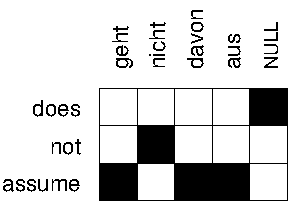
\includegraphics[scale=1]{lexical-weighting.pdf}
\end{center} \vspace{-10mm}
\maths{\begin{equation*}
\mbox{lex}(\bar{e}|\bar{f},a) = 
\prod_{i=1}^{\mbox{length}(\bar{e})} \frac{1}{|\{j|(i,j) \in a\}|} \sum_{\forall (i,j) \in a} w(e_i|f_j)
\end{equation*}}
\end{itemize}

%%%%%%%%%%%%%%%%%%%%%%%%%%%%%%%%%%%%%%%%%%%%%%%%%%%%%%%%%%%%%%%%%%%%%%%%%%%%

\slide{More Feature Functions}
\begin{itemize}
\item Language model has a bias towards short translations\\[5mm]
$\rightarrow$ word count:  \maths{$\mbox{wc}(e) = \log |{\bf e}|^\omega$}

\item We may prefer finer or coarser segmentation\\[5mm]
$\rightarrow$ phrase count  \maths{$\mbox{pc}(e) = \log |I|^\rho$}

\item Multiple language models
\item Multiple translation models
\item Other knowledge sources
\end{itemize}

%%%%%%%%%%%%%%%%%%%%%%%%%%%%%%%%%%%%%%%%%%%%%%%%%%%%%%%%%%%%%%%%%%%%%%%%%%%%

\slide{Lexicalized Reordering}
\begin{center}
\includegraphics[scale=1]{lexicalized-reordering.pdf}
\end{center} \vspace{-4mm}
\begin{itemize}
\item Distance-based reordering model is weak\\[2mm]
$\rightarrow$ learn reordering preference for each phrase pair\vspace{-3mm}
\item Three orientations types: (m) monotone, (s) swap, (d) discontinuous \vspace{-6mm}
\end{itemize}
\maths{\begin{equation*}
\begin{split}
\mbox{orientation} \in \{m, s, d\}\\
p_o(\mbox{orientation}|\bar{f},\bar{e})
\end{split}
\end{equation*}}

%%%%%%%%%%%%%%%%%%%%%%%%%%%%%%%%%%%%%%%%%%%%%%%%%%%%%%%%%%%%%%%%%%%%%%%%%%%%

\slide{Learning Lexicalized Reordering}
\begin{center}
\includegraphics[scale=1.2]{lexicalized-reordering-training.pdf}
\end{center}
\begin{itemize}
\item Collect orientation information during phrase pair extraction 
\begin{itemize}\itemsep 3mm
\item if word alignment point to the top left exists $\rightarrow$ {\bf monotone}
\item if a word alignment point to the top right exists$\rightarrow$ {\bf swap}
\item if neither a word alignment point to top left nor to the top right exists\\ $\rightarrow$  neither monotone nor swap $\rightarrow$ {\bf discontinuous}
\end{itemize}
\end{itemize}

%%%%%%%%%%%%%%%%%%%%%%%%%%%%%%%%%%%%%%%%%%%%%%%%%%%%%
%%%%%%%%%%%%%%%%%%%%%%%

\slide{Learning Lexicalized Reordering}
\begin{itemize}
\item Estimation by relative frequency
\maths{\begin{equation*}
p_o(\mbox{orientation}) = \frac{\sum_{\bar{f}} \sum_{\bar{e}} count(\mbox{orientation},\bar{e},\bar{f})}{\sum_o \sum_{\bar{f}} \sum_{\bar{e}} count(o,\bar{e},\bar{f})}
\end{equation*}}
\item Smoothing with unlexicalized orientation model \maths{$p(\mbox{orientation})$} to avoid zero probabilities for unseen orientations
\maths{\begin{equation*}
p_o(\mbox{orientation}|\bar{f},\bar{e}) = \frac{\sigma \; p(\mbox{orientation}) + count(\mbox{orientation},\bar{e},\bar{f})}{\sigma + \sum_o count(o,\bar{e},\bar{f})}
\end{equation*}}
\end{itemize}

%%%%%%%%%%%%%%%%%%%%%%%%%%%%%%%%%%%%%%%%%%%%%%%%%%%%%%%%%%%%%%%%%%%%%%%%%%%%

\slide{EM Training of the Phrase Model}
\begin{itemize}
\item We presented a heuristic set-up to build phrase translation table\\
(word alignment, phrase extraction, phrase scoring)
\item Alternative: align phrase pairs directly with EM algorithm
\begin{itemize}
\item initialization: uniform model, all \maths{$\phi(\bar{e},\bar{f})$} are the same
\item expectation step:
\begin{itemize}
\item estimate likelihood of all possible phrase alignments for all sentence pairs
\end{itemize}
\item maximization step:
\begin{itemize}
\item collect counts for phrase pairs \maths{$(\bar{e},\bar{f})$}, weighted by alignment probability
\item update phrase translation probabilties \maths{$p(\bar{e},\bar{f})$}
\end{itemize}
\end{itemize}
\item However: method easily overfits\\ (learns very large phrase pairs, spanning entire sentences)
\end{itemize}

%%%%%%%%%%%%%%%%%%%%%%%%%%%%%%%%%%%%%%%%%%%%%%%%%%%%%%%%%%%%%%%%%%%%%%%%%%%%

\slide{Summary}
\begin{itemize} \itemsep -1pt
\item Phrase Model
\item Training the model
\begin{itemize}
\item word alignment
\item phrase pair extraction
\item phrase pair scoring
\end{itemize}
\item Log linear model
\begin{itemize}
\item sub-models as feature functions
\item lexical weighting
\item word and phrase count features
\end{itemize}
\item Lexicalized reordering model
\item EM training of the phrase model
\end{itemize}

%%%%%%%%%%%%%%%%%%%%%%%%%%%%%%%%%%%%%%%%%%%%%%%%%%%%%%%%%%%%%%%%%%%%%%%%%%%%


\end{document}
